% 90-24(90쪽) — 밑면의 반지름의 길이가 5, 높이가 10 인 원뿔과 거기에 내접하는 원기둥. 스캔 화질이 낮아 TikZ 로 다시 그림.
% 원문에 있는 것만 옮긴다: 원뿔 · 원기둥 · 높이 10 · 밑면의 반지름 5 · 직각 표시(보이지 않는 선은 점선). 원기둥의 반지름은 원문 그림의 비율 그대로 그려 부피가 최대가 되는 자리를 알려 주지 않는다.
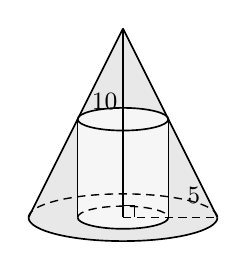
\begin{tikzpicture}[x=0.24cm, y=0.24cm, line width=0.6pt]
  % 원뿔
  \fill[gray!18] (0,10) -- (-5,0) arc(180:360:5 and 1.25) -- cycle;
  \fill[gray!18] (0,10) -- (-5,0) arc(180:0:5 and 1.25) -- cycle;
  % 원기둥(원뿔보다 앞)
  \fill[gray!7] (-2.4,0) rectangle (2.4,5.2);
  \fill[gray!7] (0,0) ellipse (2.4 and 0.6);
  \fill[gray!7] (0,5.2) ellipse (2.4 and 0.6);
  % 원뿔 윤곽
  \draw (0,10) -- (-5,0);
  \draw (0,10) -- (5,0);
  \draw (-5,0) arc(180:360:5 and 1.25);
  \draw[densely dashed, line width=0.5pt] (-5,0) arc(180:0:5 and 1.25);
  % 원기둥 윤곽
  \draw (0,5.2) ellipse (2.4 and 0.6);
  \draw (-2.4,5.2) -- (-2.4,0);
  \draw (2.4,5.2) -- (2.4,0);
  \draw (-2.4,0) arc(180:360:2.4 and 0.6);
  \draw[densely dashed, line width=0.5pt] (-2.4,0) arc(180:0:2.4 and 0.6);
  % 높이와 밑면의 반지름
  \draw[line width=0.5pt] (0,10) -- (0,0);
  \draw[densely dashed, line width=0.5pt] (0,0) -- (5,0);
  \draw[line width=0.4pt] (0,0.62) -- (0.62,0.62) -- (0.62,0);
  \node[anchor=east, inner sep=1pt, font=\small] at (-0.1,6.15) {$10$};
  \node[anchor=south, inner sep=1.5pt, font=\small] at (3.75,0.45) {$5$};
\end{tikzpicture}
